\documentclass[a4paper,french,bookmarks]{article}
\usepackage{./Structure/4PE18TEXTB}

\newlength{\littleoh}
\newlength{\littleow}
\newlength{\littlewedgeh}
\newlength{\littlewedgew}
\AtBeginDocument{\settoheight{\littleoh}{o}}
\AtBeginDocument{\settowidth{\littleow}{o}}
\AtBeginDocument{\settoheight{\littlewedgeh}{|}}
\AtBeginDocument{\settowidth{\littlewedgew}{o}}

\begin{document}

\stylizeDoc{Mathématiques}{Chapitre 15}{Limites et continuité}

Originellement, les mathématiques ont été créées comme un outil pour comprendre le monde. Les premiers savants étaient pour la plupart tout autant géomètres que physiciens ou philosophes. Le mot calcul vient après tout du latin \textit{calculus} qui signifie \textit{petit caillou}, ces derniers servant alors à représenter des animaux, des personnes, etc. pour les compter. Le monde concret cependant, diffère en bien des points des paysages abstraits atteignables en mathématiques : si aujourd'hui communément admis, les nombres négatifs, irrationnels puis \textit{imaginaires} ont successivement posé problème à des générations de mathématiciens, qui doutaient de leur existence.\\[3pt]
%
La question de la \textit{continuité} s'inscrit dans ce cadre entre mathématiques et monde réel. Dans le second, les \guill{fonctions} d'une grandeur semblent en effet toujours être \guill{lisses}, que ce soit le mouvement d'une balle qui tombe, celui de la lune autour de la terre, \dots. Dans le premier, l'on peut fabriquer des fonctions discontinues en tout point. La notion de \textit{continu} n'est pas évidente, et est intrinsèquement liée à la notion de \textit{limite}, elle-même difficile à définir. \textsc{Louis Cauchy}, déplorant le manque de rigueur des mathématiciens de son temps, donnera début \textsc{\romannumeral 19}\textsuperscript{e}~siècle cette définition de la limite dans son \textit{Cours d'analyse de l'École royale polytechnique} :
%
\begin{center}
    \begin{minipage}{0.9\linewidth}
        \qquad\quad \guill{\textit{\EBGaramond Lorsque les valeurs successivement attribuées à une même variable s'approchent indéfiniment d'une valeur 
finie, de manière à en différer aussi peu qu'on voudra, cette dernière est appelée limite de toutes les autres.}}
    \end{minipage}
\end{center}
%
Et pourtant, il écrira dans ce même ouvrage que la somme \textit{infinie} de fonctions continues est continue, ce qui pourtant est erroné (cf. les séries de \textsc{Fourier}). Il faudra attendre la moitié du \textsc{\romannumeral 19}\textsuperscript{e}~siècle pour que \textsc{Karl Weierstrass} donne une formalisation rigoureuse du concept de limite et de dérivée, que l'on utilise aujourd'hui.\\

Ce chapitre étudie les notions de limite et de continuité, notamment en généralisant aux fonctions ce qui a été vu dans le chapitre 9 sur les suites. Conformément au programme de \textsf{MP2I}, il a pour objectif avec le chapitre suivant (sur la dérivation) de démontrer \guill{\textit{les théorèmes de base relatifs aux fonctions réelles de variable réelle}}.
\initcours{}

\section{Limites}

On étudiera dans cette section les fonctions de la variable réelle et à valeurs réelles. On considérera donc dans ce qui suit une partie $X \in \bdR$ et une fonction $f \in \bcF(X, \bdR)$.

\subsection{Voisinage}

Les voisinages permettent de considérablement simplifier l'étude locale des fonctions réelles. On donne donc ci-dessous, sans rentrer dans tous les détails de la topologie, une définition des voisinages sur $\bdR$. On commence alors par définir le voisinage d'un réel $\alpha$ :

\begin{definition}{Voisinage d'un réel}{}
    Soit $\alpha \in \bdR$ et une partie $V \subset \bdR$. On dit que \hg{$V$ est un voisinage de $a$} lorsque
    %
    \[\hg{\exists \epsilon \in \bdRp, \qquad \left]\alpha - \epsilon, \alpha + \epsilon\right[ \subset V}\]
\end{definition}

\begin{hpnote}
       Le voisinage d'un réel $\alpha$ sur $\bdR$ un donc un sous-ensemble $V$ de $\bdR$ tel qu'il existe une boule \textit{ouverte} de centre $\alpha$ et de rayon $\epsilon$ - notée $B(\alpha, \epsilon)$ - entièrement incluse dans $V$. Cette idée de \guill{boule} permet en fait de généraliser la notion de voisinage à tout espace métrique, notamment à $\bdR^n$ :

        \begin{enumerate}
           \itt Sur la droite $\bdR$, les boules sont les intervalles : $B(\alpha, \epsilon) = \{ x \in \bdR \mid \mod{x - \alpha} < \epsilon\} = \left]\alpha - \epsilon, \alpha + \epsilon\right[$.
    
          \itt Dans le plan $\bdR^2 \cong \bdC$, les boules sont des disques $B(\alpha, \epsilon) = \{ z \in \bdC \mid \mod{z - \alpha} < \epsilon\}$
    
          \itt Dans l'espace $\bdR^3$, les boules sont des\dots \ \ boules.
        \end{enumerate}

        En général, une fois un espace métrique $E$ muni de sa distance $d :     \begin{array}[t]{ccc}
           E\times E &\to &\bdR_+  \\
          (x,y) &\mapsto &d(x, y)
        \end{array}$, on peut définir la boule ouverte $B(\alpha, \epsilon)$ et fermée $\overline{B}(\alpha, \epsilon)$, de centre $\alpha$ et de rayon $\epsilon$ comme :
        %
        \[ B(\alpha, \epsilon) = \{ x \in E \mid d(x, y) < \epsilon\} \qquad\qquad \overline{B}(\alpha, \epsilon) = \{ x \in E \mid d(x, y) \leq \epsilon\}\]
        %
        La fonction $d$ se comprend intuitivement : sur $\bdR$ il s'agit de la valeur absolue $\mod{x-y}$, sur $\bdC$ du module $\mod{x -y}$, sur $\bdR^n$ de la norme $\norm{\vec u - \vec v}$, \dots. Le voisinage d'un point d'un espace métrique est donc un sous-ensemble contenant une boule ouverte centrée en ce point. \textit{En fait, on définit en topologie le voisinage d'un point comme étant une partie contenant un \guill{ouvert} contenant ce point}.
\end{hpnote}

On peut de même définir une notion de voisinage de $+\infty$ et $-\infty$ :

\begin{definition}{Voisinage de l'infini}{}
    \begin{enumerate}
        \ithand Soit une partie $V \subset \bdR$. On dit que \hg{$V$ est un voisinage de $+\infty$} lorsque
        %
        \[\hg{\exists M \in \bdR, \qquad V = ]M, +\infty[} \]
        
        \ithand On dit de plus que \hg{$V$ est un voisinage de $-\infty$} lorsque
        %
        \[ \hg{\exists m \in \bdR, \qquad V = ]-\infty, m[} \]
    \end{enumerate}
\end{definition}

On pourra donc, en regroupant ces trois cas, considérer un voisinage de $\alpha \in \overline\bdR$ quelconque, pouvant donc être fini ($\alpha \in \bdR$), comme infini ($\alpha = +\infty$ ou $\alpha = -\infty$). On définit alors, par praticité, l'ensemble des voisinages de $\alpha$ :

\begin{definition}{Ensemble des voisinages}{}
    Soit $\alpha \in \overline\bdR$. On désigne par \hg{$\bcV(\alpha)$ l'ensemble des voisinages de $\alpha$}.
\end{definition}

Les voisinages peuvent être visualisées de manière très simple :

\begin{center}
\begin{minipage}{0.3\linewidth}
    \centering
    
    Voisinage de $\alpha \in \bdR$ :
    \begin{tikzpicture}
        \draw[->] (0,0) -- (4,0);
    \end{tikzpicture}
    
\end{minipage}
\begin{minipage}{0.03\linewidth}
\hfill
\end{minipage}
\begin{minipage}{0.3\linewidth}
    \center
    Voisinage de $-\infty$ :
    
\end{minipage}
\begin{minipage}{0.03\linewidth}
\hfill
\end{minipage}
\begin{minipage}{0.3\linewidth}
    Voisinage de $+\infty$ :
    
\end{minipage}
\end{center}

Vient alors un premier aspect intéressant des voisinages : en effet, là où une fonction respecte une propriété en un certain point $a$, il est courant que cette propriété soit aussi valide pour les points situés \guill{autour de $a$}. Plus précisément :

\begin{definition}{Propriété vérifiée au voisinage}{}
    Soit $D \subset \bdR$ et $f: D \to \bdR$. On dit que \bf{$f$ vérifie la propriété $P$ au voisinage de $a \in \overline\bdR$} si et seulement si
    
    \[ \hg{\exists V \in \bcV(a), \qquad \text{tel que} \qquad \forall x \in D \cap V, \qquad f(x) \ \text{vérifie} \ P}\]
\end{definition}

\begin{example}{}{}
    \begin{enumerate}
        \ithand $x \mapsto \dfrac{1}{x}$ est \hg{bornée au voisinage de $1$, $+\infty$ et $-\infty$}.
        
        \ithand $\sin$ est \hg{croissante au voisinage de $0$} (en effet $\sin$ est croissante sur $\left[-\sfrac{\pi}{2}, \sfrac{\pi}{2}\right]$.
        
        \ithand $x \mapsto \lfloor x \rfloor$ (partie entière) est \hg{constante au voisinage de tout point $a \in \bcR \backslash \bdZ$}.
    \end{enumerate}
\end{example}

\subsection{Limite finie}

Pour une suite $\suite{u_n} \in \bdK^\bdN$, on avait défini les limites de la façon suivante :

\[ \lim\limits_{n \to +\infty} u_n = l \quad \iff \quad u_n \lima{n \to +\infty} l \qquad \iff \qquad \forall \epsilon \in \bdRp, \quad \exists N \in \bdN, \quad \forall n \in \bdN,\quad n \geq N \implies \mod{u_n - l} \leq \epsilon\]

On peut alors généraliser cette définition pour les fonctions :

\subsection{Limite infinie}

On s'intéresse au cas où $l = +\infty$ ou $l = -\infty$. On est en fait face à trois cas :



\begin{definition}{Limite d'une fonction}{}
    Soit $D \subset \bdR$ et $f : D \to \bdR$. On dit que \bf{ $f(x)$ admet une limite $l \in \overline\bdR$ lorsque $x$ tends vers $a \in \overline\bdR \cap D$} si et seulement si
    %\[ \hg{\forall \epsilon \in \bdRp,\quad \exists V \in \bcV(a),\quad \forall x \in D \cap V, \qquad \mod{f(x) - l} \leq \epsilon}\]
    
    \[\hg{\forall V \in \bcV(l),\qquad \exists W \in \bcV(a),\qquad \forall x \in D,\qquad x \in W \implies f(x) \in V}\]
\end{definition}

$u_n = O(n^2) = \mathcal{O}(n^2)$ et $u_n = o(n^3) = \resizebox{\littleow}{\littleoh}{$\mathcal O$}(n^3)$.


\begin{form}{Notation ?}{}
\[ n \wedge m \qquad\qquad\text{ou}\qquad\qquad n \, \resizebox{0.95\littlewedgew}{0.4\littlewedgeh}{$\wedge$}\,  m\]
\end{form}

\begin{center}
    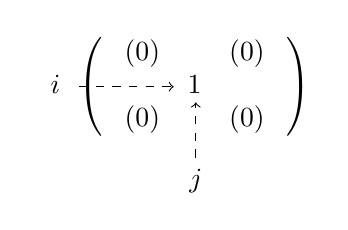
\begin{tikzpicture}
\node{$\begin{array}{c}
    \text{} \\ i \\ \text{}
\end{array}\left(\vphantom{\begin{array}{c}
    1\\ 2\\ 3
\end{array}}\right.\begin{array}{ccc}
    (0) & & (0) \\
     & 1 & \\
     (0) &  & (0)
\end{array}\left.\vphantom{\begin{array}{c}
    1\\ 2\\ 3
\end{array}}\right)$};
\draw[dashed, ->] (-1.2, 0) -- (0, 0);
\node at (0.28, -1.2) {$j$};
\draw[dashed, ->] (0.28, -0.9) -- (0.28, -0.2);
\end{tikzpicture}
\end{center}

\[\left(\begin{array}{ccccc}
    0\tikzmarknode{0top}{} & 1 & \cdots & \cdots & 1  \\
    1 &  & \ddots & & \vdots \\
    \vdots & \ddots &  & \ddots & \vdots \\
    \vdots & & \ddots &  & 1\\
    1 & \cdots & \cdots & 1 & \tikzmarknode{0bottom}{0}
\end{array}\right)\]
\begin{tikzpicture}[overlay,remember picture,>=Stealth]
  \draw[-] (0top) -- (0bottom);
\end{tikzpicture}

\newpage
\begin{theorem}{}
    Soit $f : ] a, b [ \to \bdR$ avec $a < b$ et $(a, b) \in \bdR2$.
    
    Si $f$ est monotone sur $]a, b[$, alors $f$ possède une limite à droite en $a$ et une limite à gauche en $b$. 
\end{theorem}

\newpage

\begin{theorem}{Lien entre injectivité et stricte monotonie}{}

    Soit $f \in \bcC(I, \bdR)$. On a équivalence entre

    \begin{enumerate}[label=(\roman*)]
       \item $f$ est injective
       \item $f$ est strictement monotone
    \end{enumerate}
    
\end{theorem}

\demoth{
    Soit $f \in \bcC(I, \bdR)$. Montrons $\boxed{(ii) \implies (i)}$\footnote{En vérité, cette implication ne nécessite pas la continuité de $f$.}.
    
    Si $f$ est strictement monotone sur $I$, on peut déjà considérer deux points $(a, b) \in I^2$, avec $a \neq b$ ; alors par stricte monotonie, on a :
    
    \[ a \neq b \implies a > b \lor a < b \implies f(a) > f(b) \lor f(a) < f(b) \implies f(a) \neq f(b)\]
    
    Donc $f$ est injective. Montrons maintenant $\boxed{(ii) \impliedby (i)}$. Supposons $f$ injective. Soient $(a, b) \in I^2$ tels que $a < b$. Supposons (par exemple) que $f(a) < f(b)$. Donnons-nous $(x, y) \in I^2$ tels que $x < y$. Montrons que $f(x) < f(y)$. On introduit :
    
    \[ \varphi : \begin{array}[t]{ccc}
        [0, 1] &\to& \bdR  \\
        t &\mapsto& f(tx + (1-t)a) - f(ty+(1-t)b) 
    \end{array}\]
    
    On a $\varphi(0) = f(a) - f(b) < 0$, et $\varphi(1) = f(x) - f(y)$. Par composée et somme, $\varphi$ et continue sur $[0, 1]$ (car $f$ continue sur $I$). Par l'absurde, si $\varphi(1) \geq 0$, alors le TVI donne l'existence d'un $t_0 \in [0, 1]$ tel que $\varphi(t_0) = 0$. Donc :
    
    \[ f(t_0x+(1-t_0)a) = f(t_0y + (1-t_0)b)\]
     
    Ce qui est absurde car $f$ est injective. Donc $\varphi(1) < 0$, soit $f(x) < f(y)$. Une même discussion s'opère dans le cas $f(a) > f(b)$. On a donc montré que $f$ est strictement monotone sur $I$.
}

\begin{theorem}{Bijection continue}{}
    Soit $f \in \bcC(I, \bdR)$ et $f$ strictement monotone sur $I$. Alors :
    
    \begin{enumerate}[label=(\roman*)]
        \item $f$ réalise une bijection de $I$ dans $f(I)$
        \item L'ensemble $f(I)$ est un intervalle de même nature que $I$.
        \item La réciproque $f^{-1} : f(I) \to I$ est continue et de même monotonie que $f$.
    \end{enumerate}

\end{theorem}

\end{document}